\clearpage
\section{Effects from Initial State Radiation}
\label{app:isr}
The transverse polarization parameters, $\alpha_0$ and $\sin\Delta_0$, are correlated to $G_E$ and $G_M$ which depends on the collision energies. The Initial State Radiation (ISR) could cause migration effects on the center-of-mass energies, especially for high energy points. The total energy of ISR gammas are checked using the PHSP signal MC samples at $\sqrt{s} = 4.918\gev/c^2$ as shown in Figure~\ref{fig:isr_energy}, which has a long tail to around 350 MeV. However, events with high ISR effects are highly suppressed by the $\Delta E$ and $\mbc$ requirements in the nominal analysis. The effects from ISR are estimated by varying the $\Delta E$ or $\mbc$ requirements and comparing the alternative amplitude analysis results to the nominal one.

\begin{figure}[H]\centering
    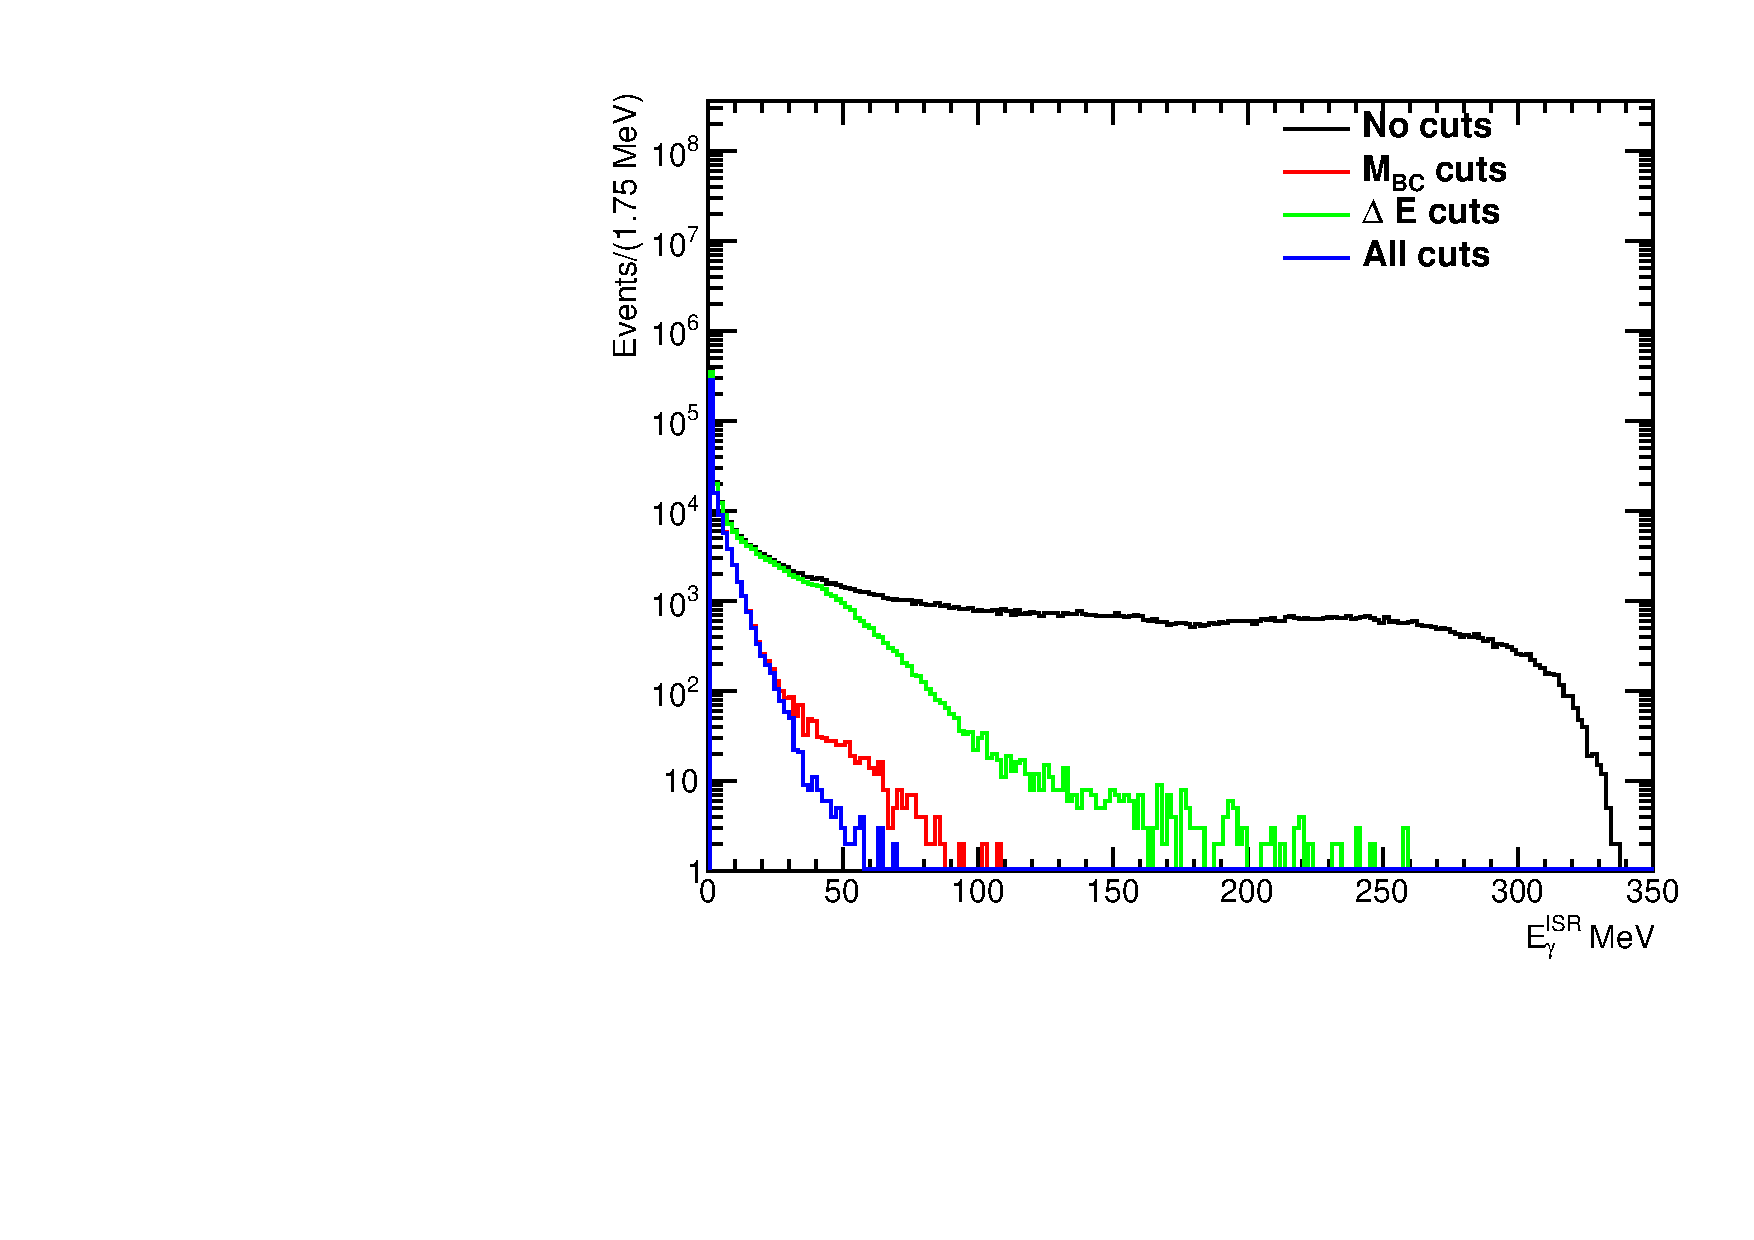
\includegraphics[width=0.45\textwidth]{figure/isr_effects/output_4914_phsp_ISR_gamma_E.pdf}
    \caption{Distribution of total energy of ISR gammas from truth information at $\sqrt{s} = 4.918\gev$.}
\label{fig:isr_energy}
\end{figure}

A total six alternative $\Delta E$ ($\mbc$) requirements are test, three of them are obtained by narrowing the nominal one by a fraction of 15\%, 10\% and 5\% around 0 ($m_{\lcp}$), while others are obtained by broadening by 5\%, 10\% and 15\%. With each updated $\Delta E$ ($\mbc$) requirement, the entire analysis procedure are performed to determine the transverse polarization parameters. The updated background fractions for each energy points are listed in Table~\ref{tab:bkg_frac_deltaE} and Table~\ref{tab:bkg_frac_mbc} for varied $\Delta E$ and $\mbc$ requirement windows, respectively. The amplitude analysis is performed using the updated inputs and the comparison are shown in Figure~\ref{fig:comparison_deltaE} and~\ref{fig:comparison_mBC} for $\sqrt{s} = 4.918$ and 4.950$\gev/c^2$. The maximum difference between nominal and alternative requirements are much smaller than the statistical uncertainties, which indicates the ISR effects on polarization measurement should be small.  

\begin{table}[H]
    \centering
    \caption{Background fractions in $\mbc$ signal region with varied $\Delta E$ requirements. }
    \label{tab:bkg_frac_deltaE}
    \resizebox{\textwidth}{!}{
    \begin{tabular}{ccccccccc}
    \hline\hline
    Dataset  & Nominal (\%) & -15\% & -10\% & -5\% & 5\% & 10\% & 15\%\\\hline
    4600 & 5.1$\pm$0.2 & 4.4$\pm$0.2 & 4.7$\pm$0.2 & 4.9$\pm$0.2 & 5.3$\pm$0.2 & 5.5$\pm$0.2 & 5.9$\pm$0.2 \\
    4612 & 6.5$\pm$0.5 & 5.3$\pm$3.6 & 5.8$\pm$0.5 & 5.1$\pm$0.0 & 6.6$\pm$0.5 & 6.7$\pm$0.4 & 6.8$\pm$0.5 \\
    4626 & 6.1$\pm$0.2 & 4.9$\pm$0.0 & 5.3$\pm$0.0 & 5.7$\pm$0.2 & 6.5$\pm$0.2 & 6.8$\pm$0.1 & 7.1$\pm$0.2 \\
    4640 & 5.9$\pm$0.2 & 4.7$\pm$0.2 & 5.1$\pm$0.2 & 5.5$\pm$0.2 & 6.4$\pm$0.2 & 6.7$\pm$0.2 & 7.0$\pm$0.2 \\
    4660 & 6.4$\pm$0.2 & 5.3$\pm$0.2 & 5.7$\pm$0.2 & 6.0$\pm$0.2 & 6.8$\pm$0.2 & 7.2$\pm$0.2 & 7.6$\pm$0.2 \\
    4680 & 7.1$\pm$0.1 & 6.0$\pm$0.1 & 6.4$\pm$0.1 & 6.7$\pm$0.1 & 7.4$\pm$0.1 & 7.8$\pm$0.1 & 8.1$\pm$0.1 \\
    4700 & 7.5$\pm$0.2 & 6.3$\pm$0.2 & 6.7$\pm$0.2 & 7.1$\pm$0.2 & 7.9$\pm$0.2 & 8.3$\pm$0.2 & 8.7$\pm$0.2 \\
    4740 & 9.7$\pm$0.6 & 8.4$\pm$0.5 & 8.7$\pm$0.5 & 9.1$\pm$0.5 & 10.2$\pm$0.6 & 10.5$\pm$0.6 & 11.1$\pm$0.6 \\
    4750 & 9.1$\pm$0.4 & 7.4$\pm$0.3 & 7.9$\pm$0.3 & 8.4$\pm$0.3 & 9.5$\pm$0.4 & 10.0$\pm$0.4 & 10.4$\pm$0.4 \\
    4780 & 8.2$\pm$0.3 & 6.8$\pm$0.3 & 7.3$\pm$0.3 & 7.8$\pm$0.3 & 8.7$\pm$0.3 & 9.2$\pm$0.3 & 9.6$\pm$0.3 \\
    4840 & 10.7$\pm$0.4 & 8.7$\pm$0.4 & 9.3$\pm$0.4 & 9.9$\pm$0.4 & 11.4$\pm$0.4 & 12.0$\pm$0.4 & 12.5$\pm$0.5 \\
    4914 & 8.3$\pm$0.6 & 6.9$\pm$0.5 & 7.6$\pm$0.5 & 8.0$\pm$0.5 & 8.9$\pm$0.5 & 9.5$\pm$0.6 & 10.1$\pm$0.6 \\
    4946 & 9.2$\pm$0.7 & 7.7$\pm$0.7 & 7.9$\pm$0.6 & 8.2$\pm$0.7 & 9.5$\pm$0.7 & 10.0$\pm$0.7 & 10.6$\pm$0.8 \\
    \hline\hline
    \end{tabular}
    }
\end{table}

\begin{table}[H]
    \centering
    \caption{Background fractions in varied $\mbc$ signal regions. }
    \label{tab:bkg_frac_mbc}
    \resizebox{\textwidth}{!}{
    \begin{tabular}{ccccccccc}
    \hline\hline
    Dataset  & Nominal (\%) & -15\% & -10\% & -5\% & 5\% & 10\% & 15\%\\\hline
    4600 & 5.1$\pm$0.2 & 4.4$\pm$0.2 & 4.7$\pm$0.2 & 4.9$\pm$0.2 & 5.3$\pm$0.2 & 5.5$\pm$0.2 & 5.9$\pm$0.2 \\
    4612 & 6.5$\pm$0.5 & 5.3$\pm$3.6 & 5.8$\pm$0.5 & 5.1$\pm$0.0 & 6.6$\pm$0.5 & 6.7$\pm$0.4 & 6.8$\pm$0.5 \\
    4626 & 6.1$\pm$0.2 & 4.9$\pm$0.0 & 5.3$\pm$0.0 & 5.7$\pm$0.2 & 6.5$\pm$0.2 & 6.8$\pm$0.1 & 7.1$\pm$0.2 \\
    4640 & 5.9$\pm$0.2 & 4.7$\pm$0.2 & 5.1$\pm$0.2 & 5.5$\pm$0.2 & 6.4$\pm$0.2 & 6.7$\pm$0.2 & 7.0$\pm$0.2 \\
    4660 & 6.4$\pm$0.2 & 5.3$\pm$0.2 & 5.7$\pm$0.2 & 6.0$\pm$0.2 & 6.8$\pm$0.2 & 7.2$\pm$0.2 & 7.6$\pm$0.2 \\
    4680 & 7.1$\pm$0.1 & 6.0$\pm$0.1 & 6.4$\pm$0.1 & 6.7$\pm$0.1 & 7.4$\pm$0.1 & 7.8$\pm$0.1 & 8.1$\pm$0.1 \\
    4700 & 7.5$\pm$0.2 & 6.3$\pm$0.2 & 6.7$\pm$0.2 & 7.1$\pm$0.2 & 7.9$\pm$0.2 & 8.3$\pm$0.2 & 8.7$\pm$0.2 \\
    4740 & 9.7$\pm$0.6 & 8.4$\pm$0.5 & 8.7$\pm$0.5 & 9.1$\pm$0.5 & 10.2$\pm$0.6 & 10.5$\pm$0.6 & 11.1$\pm$0.6 \\
    4750 & 9.1$\pm$0.4 & 7.4$\pm$0.3 & 7.9$\pm$0.3 & 8.4$\pm$0.3 & 9.5$\pm$0.4 & 10.0$\pm$0.4 & 10.4$\pm$0.4 \\
    4780 & 8.2$\pm$0.3 & 6.8$\pm$0.3 & 7.3$\pm$0.3 & 7.8$\pm$0.3 & 8.7$\pm$0.3 & 9.2$\pm$0.3 & 9.6$\pm$0.3 \\
    4840 & 10.7$\pm$0.4 & 8.7$\pm$0.4 & 9.3$\pm$0.4 & 9.9$\pm$0.4 & 11.4$\pm$0.4 & 12.0$\pm$0.4 & 12.5$\pm$0.5 \\
    4914 & 8.3$\pm$0.6 & 6.9$\pm$0.5 & 7.6$\pm$0.5 & 8.0$\pm$0.5 & 8.9$\pm$0.5 & 9.5$\pm$0.6 & 10.1$\pm$0.6 \\
    4946 & 9.2$\pm$0.7 & 7.7$\pm$0.7 & 7.9$\pm$0.6 & 8.2$\pm$0.7 & 9.5$\pm$0.7 & 10.0$\pm$0.7 & 10.6$\pm$0.8 \\
    \hline\hline
    \end{tabular}
}
\end{table}

\begin{figure}[h]\centering
    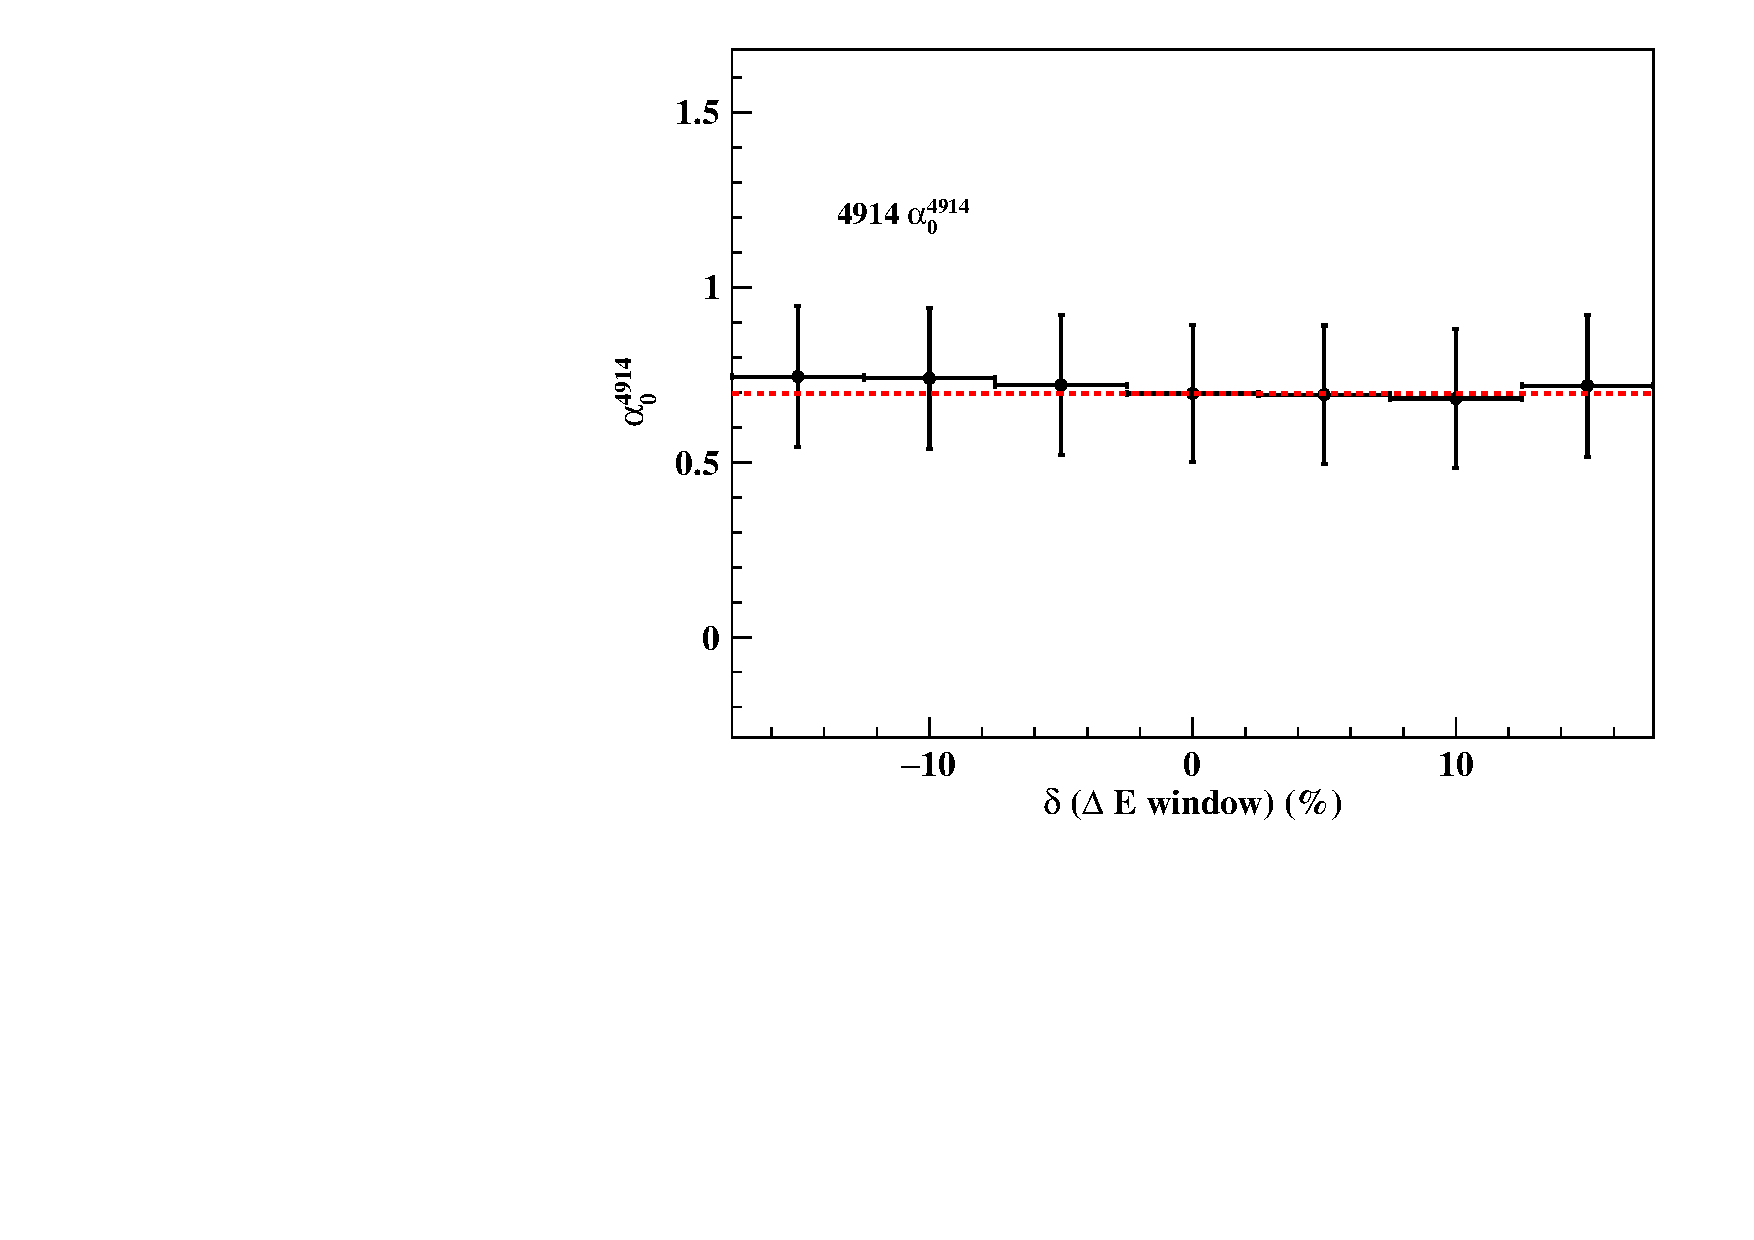
\includegraphics[width=0.40\textwidth]{figure/isr_effects/pwa_fit/output_resutls_deltaE_alpha_4914.pdf}
    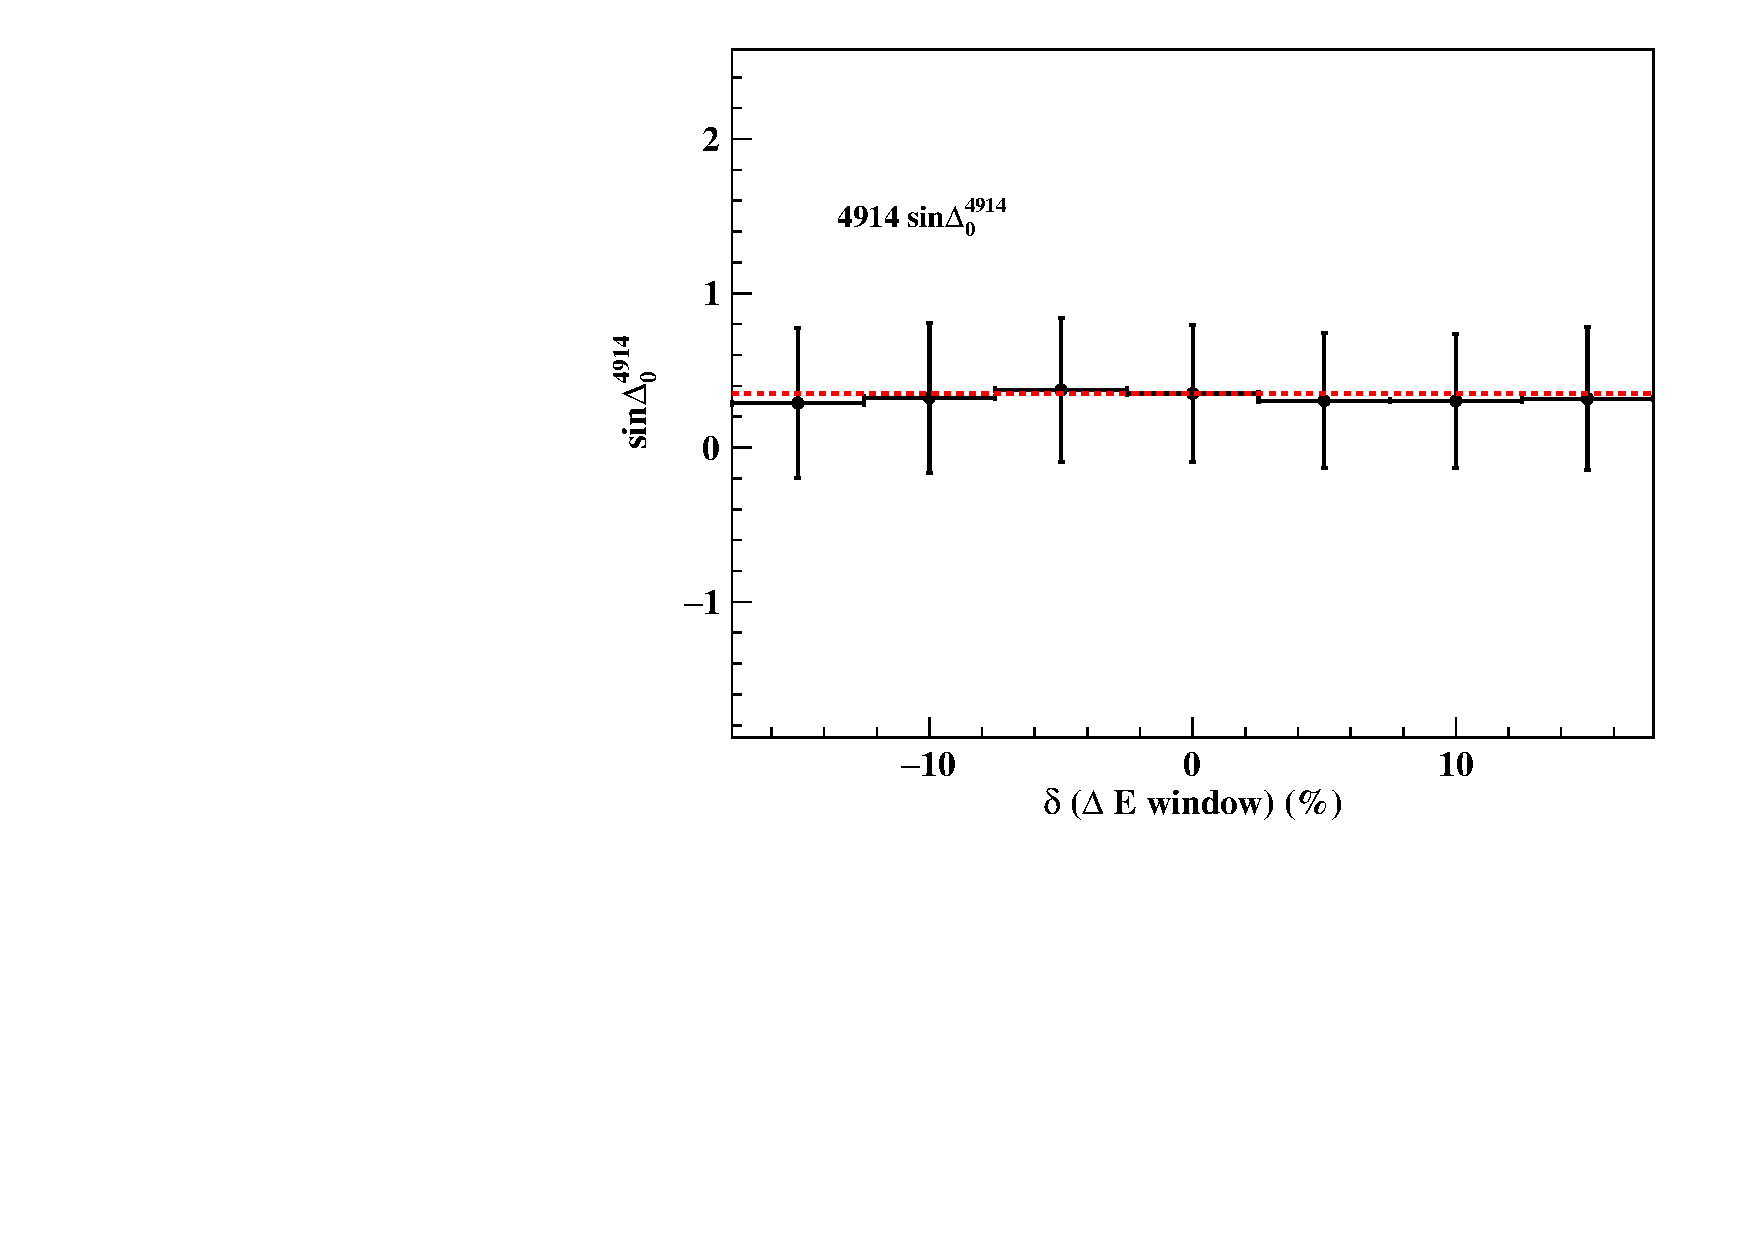
\includegraphics[width=0.40\textwidth]{figure/isr_effects/pwa_fit/output_resutls_deltaE_delta_4914.pdf} \\
    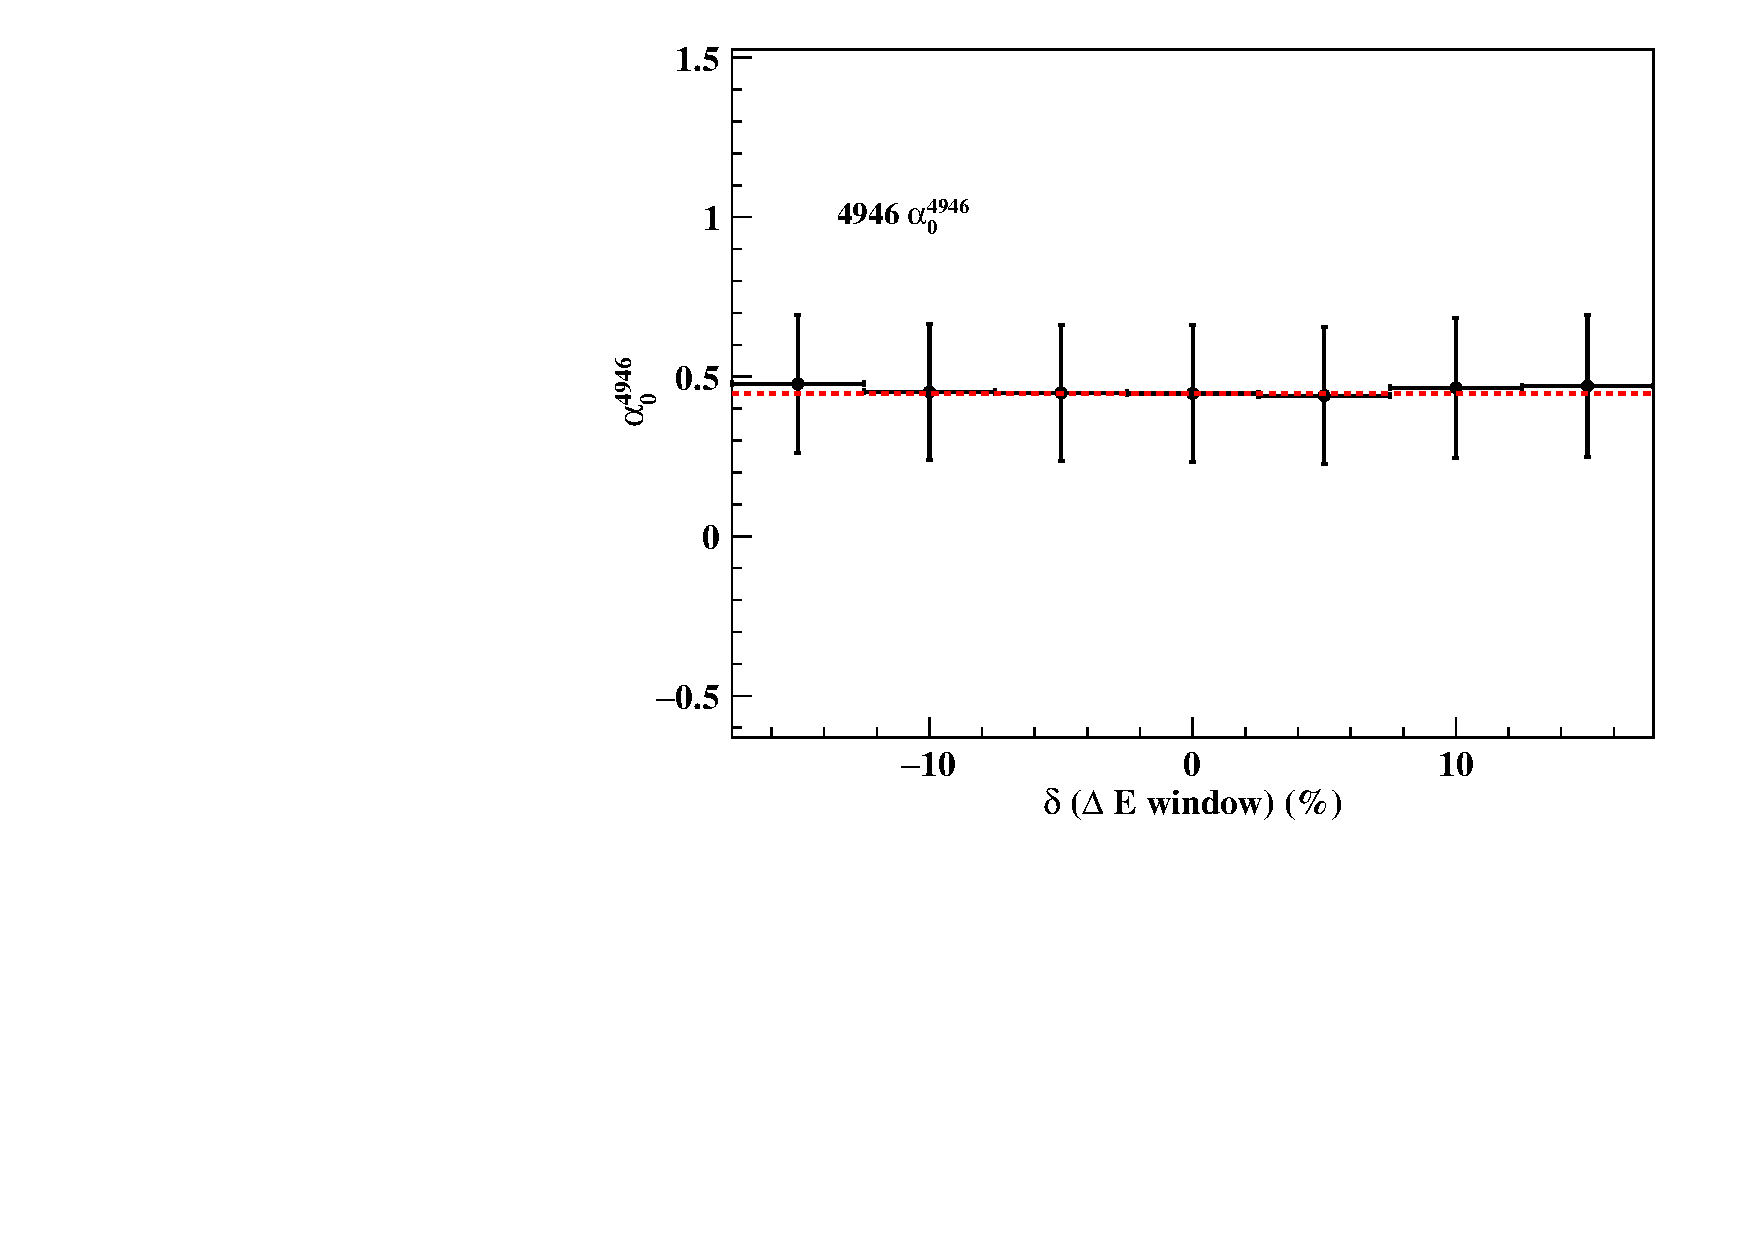
\includegraphics[width=0.40\textwidth]{figure/isr_effects/pwa_fit/output_resutls_deltaE_alpha_4946.pdf}
    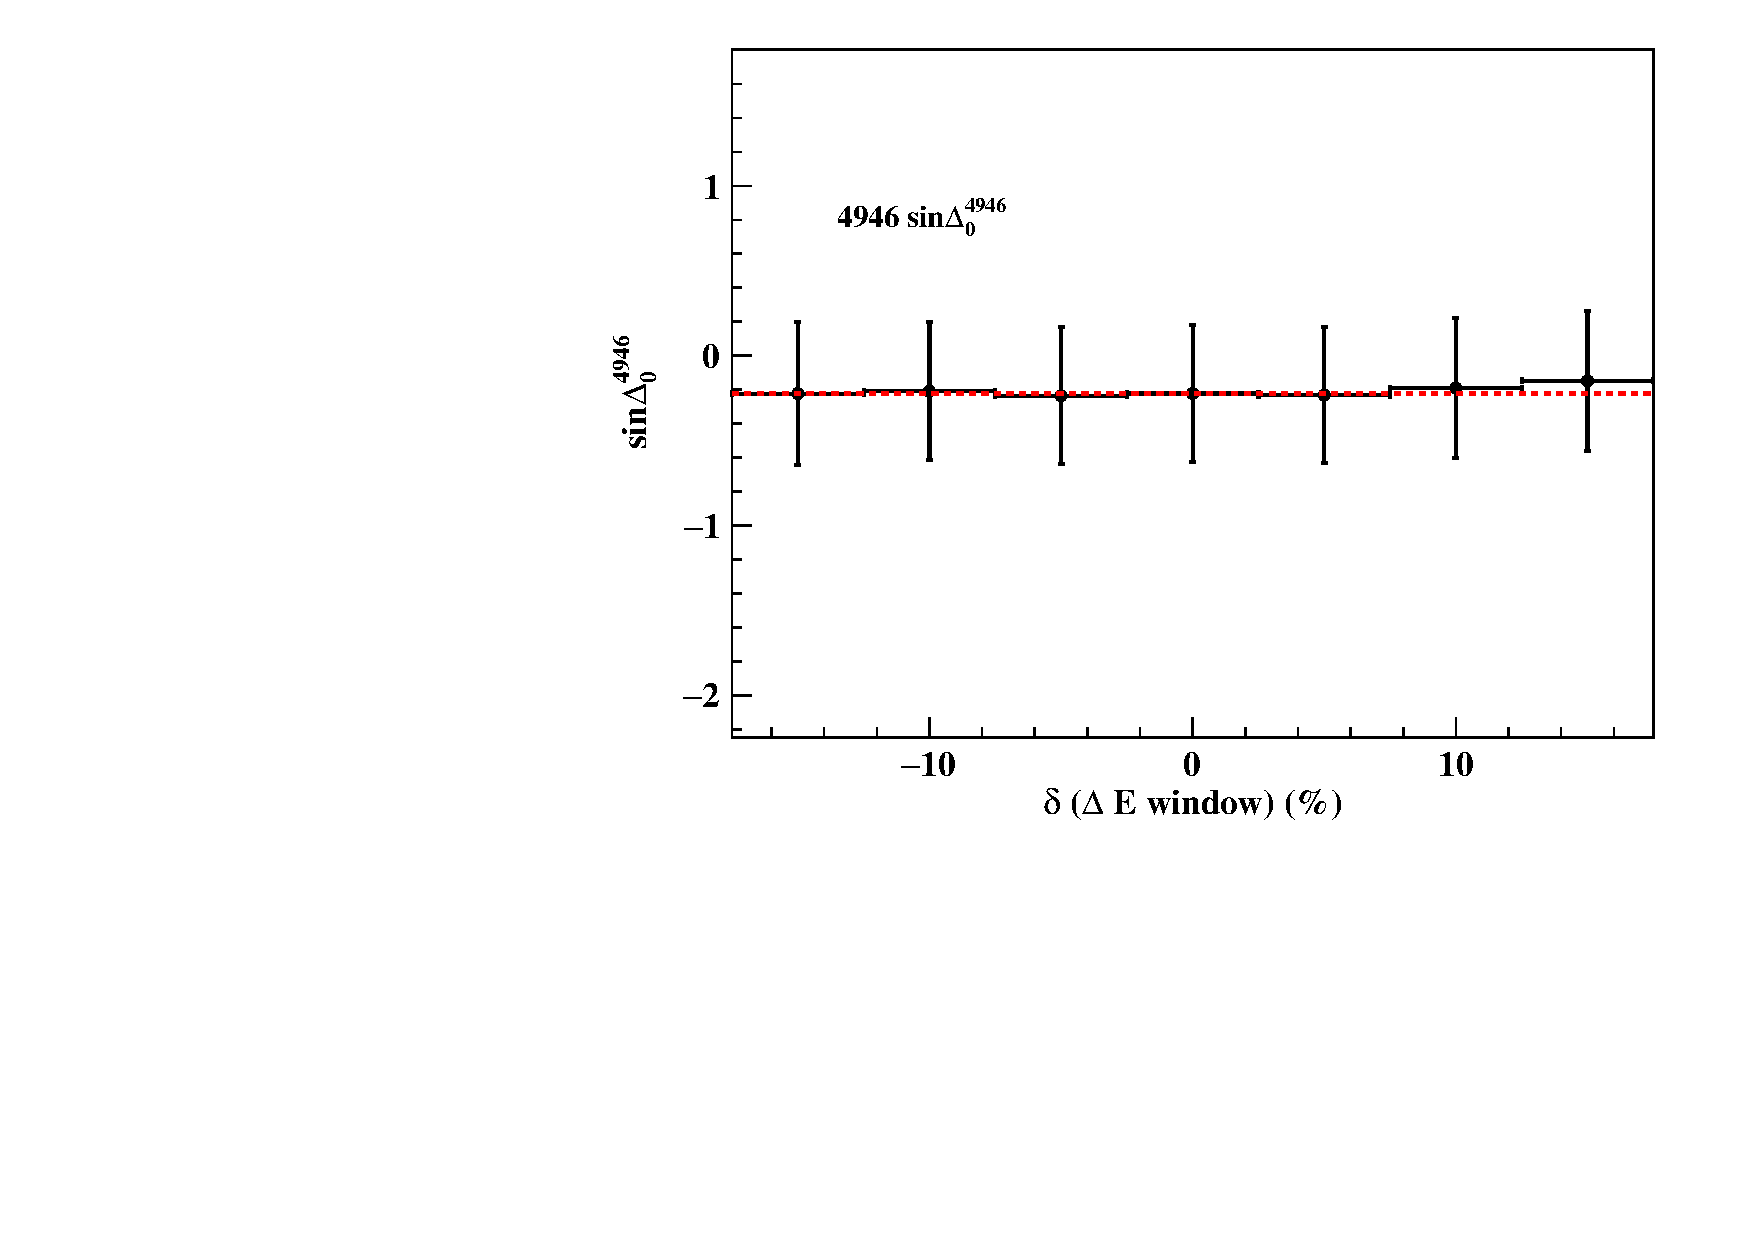
\includegraphics[width=0.40\textwidth]{figure/isr_effects/pwa_fit/output_resutls_deltaE_delta_4946.pdf}
    \caption{Comparison of $\alpha_0$ (left) and $\sin\Delta_0$ between nominal and alternative $\Delta E$ requirements at $sqrt{s} = 4.918\gev/c^2$ (top) and $\sqrt{s} = 4.950\gev/c^2$ (bottom). The middle points represent the nominal results and error bars are statistical uncertainties.}
\label{fig:comparison_deltaE}
\end{figure}

\begin{figure}[h]\centering
    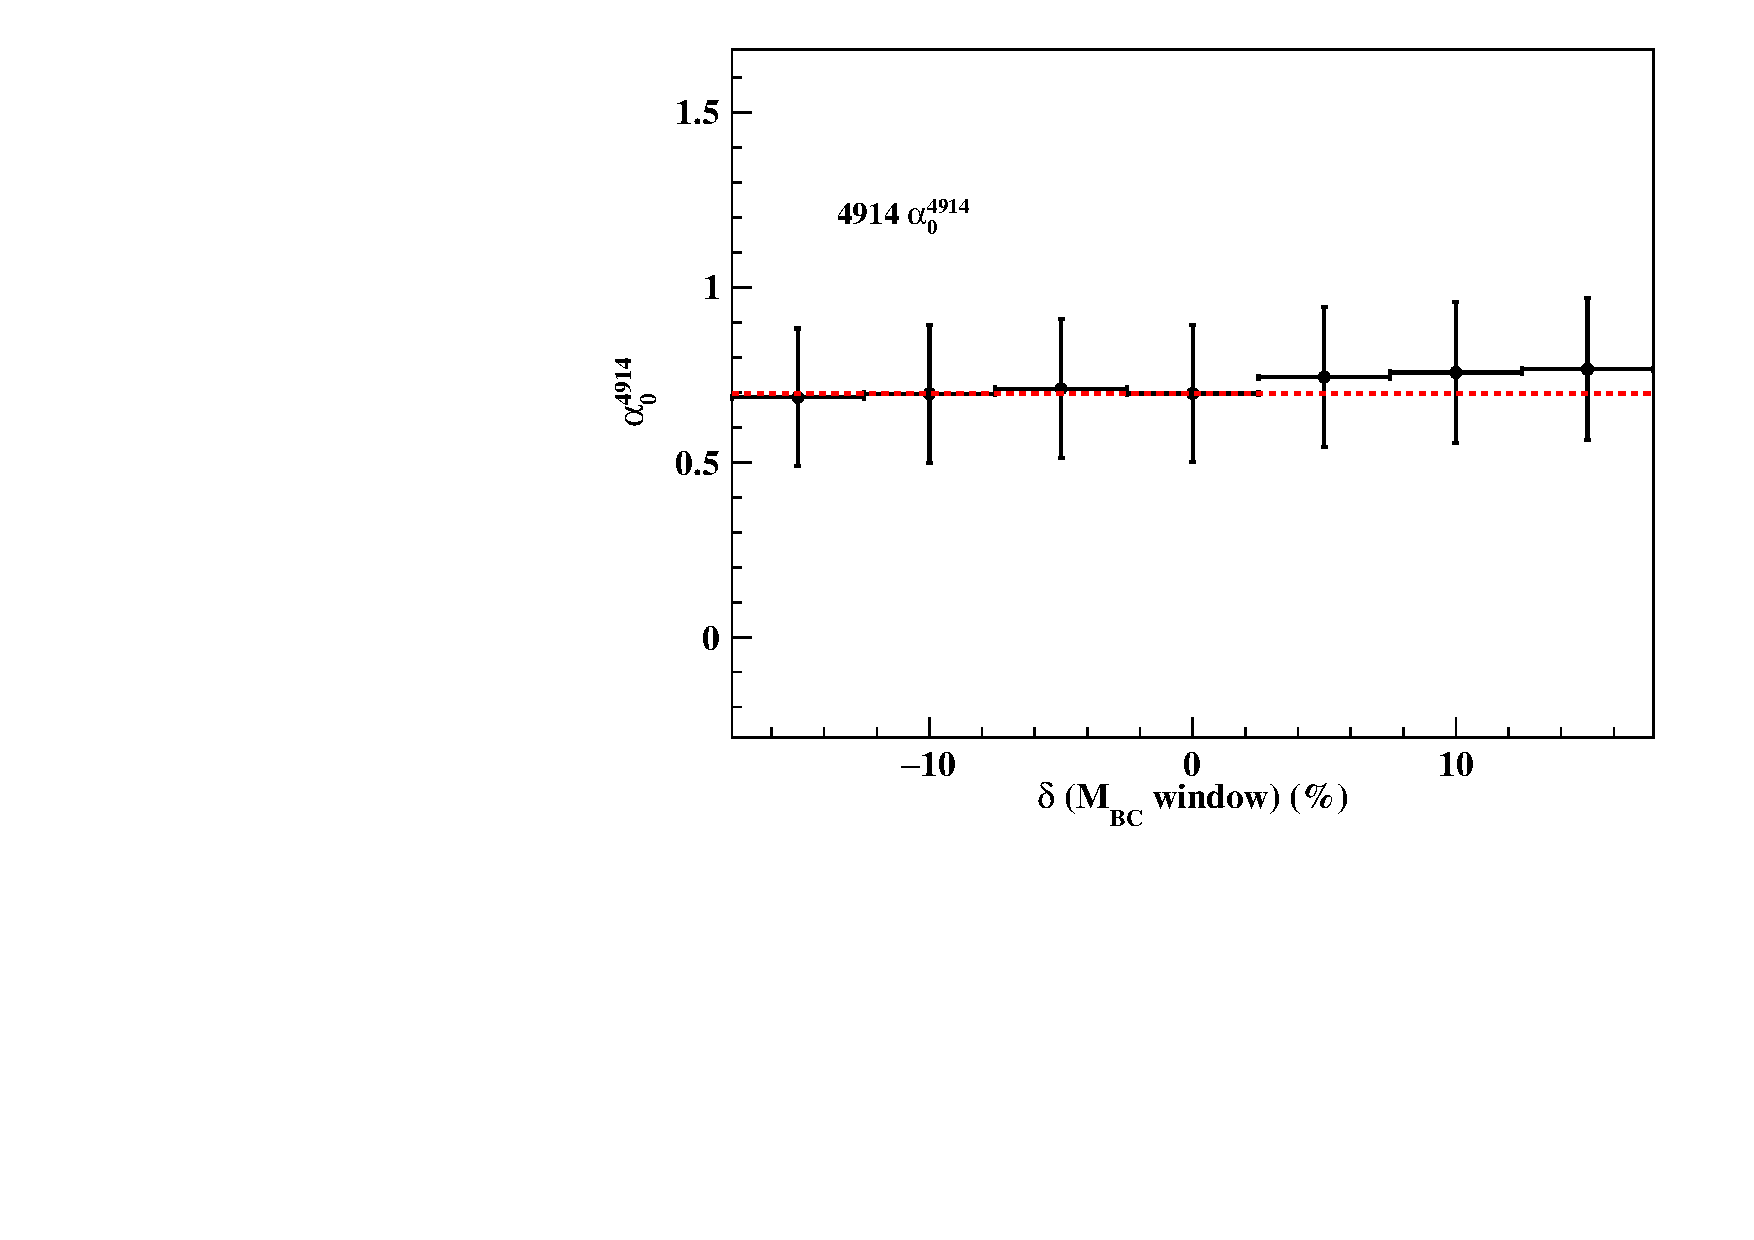
\includegraphics[width=0.40\textwidth]{figure/isr_effects/pwa_fit/output_resutls_mBC_alpha_4914.pdf}
    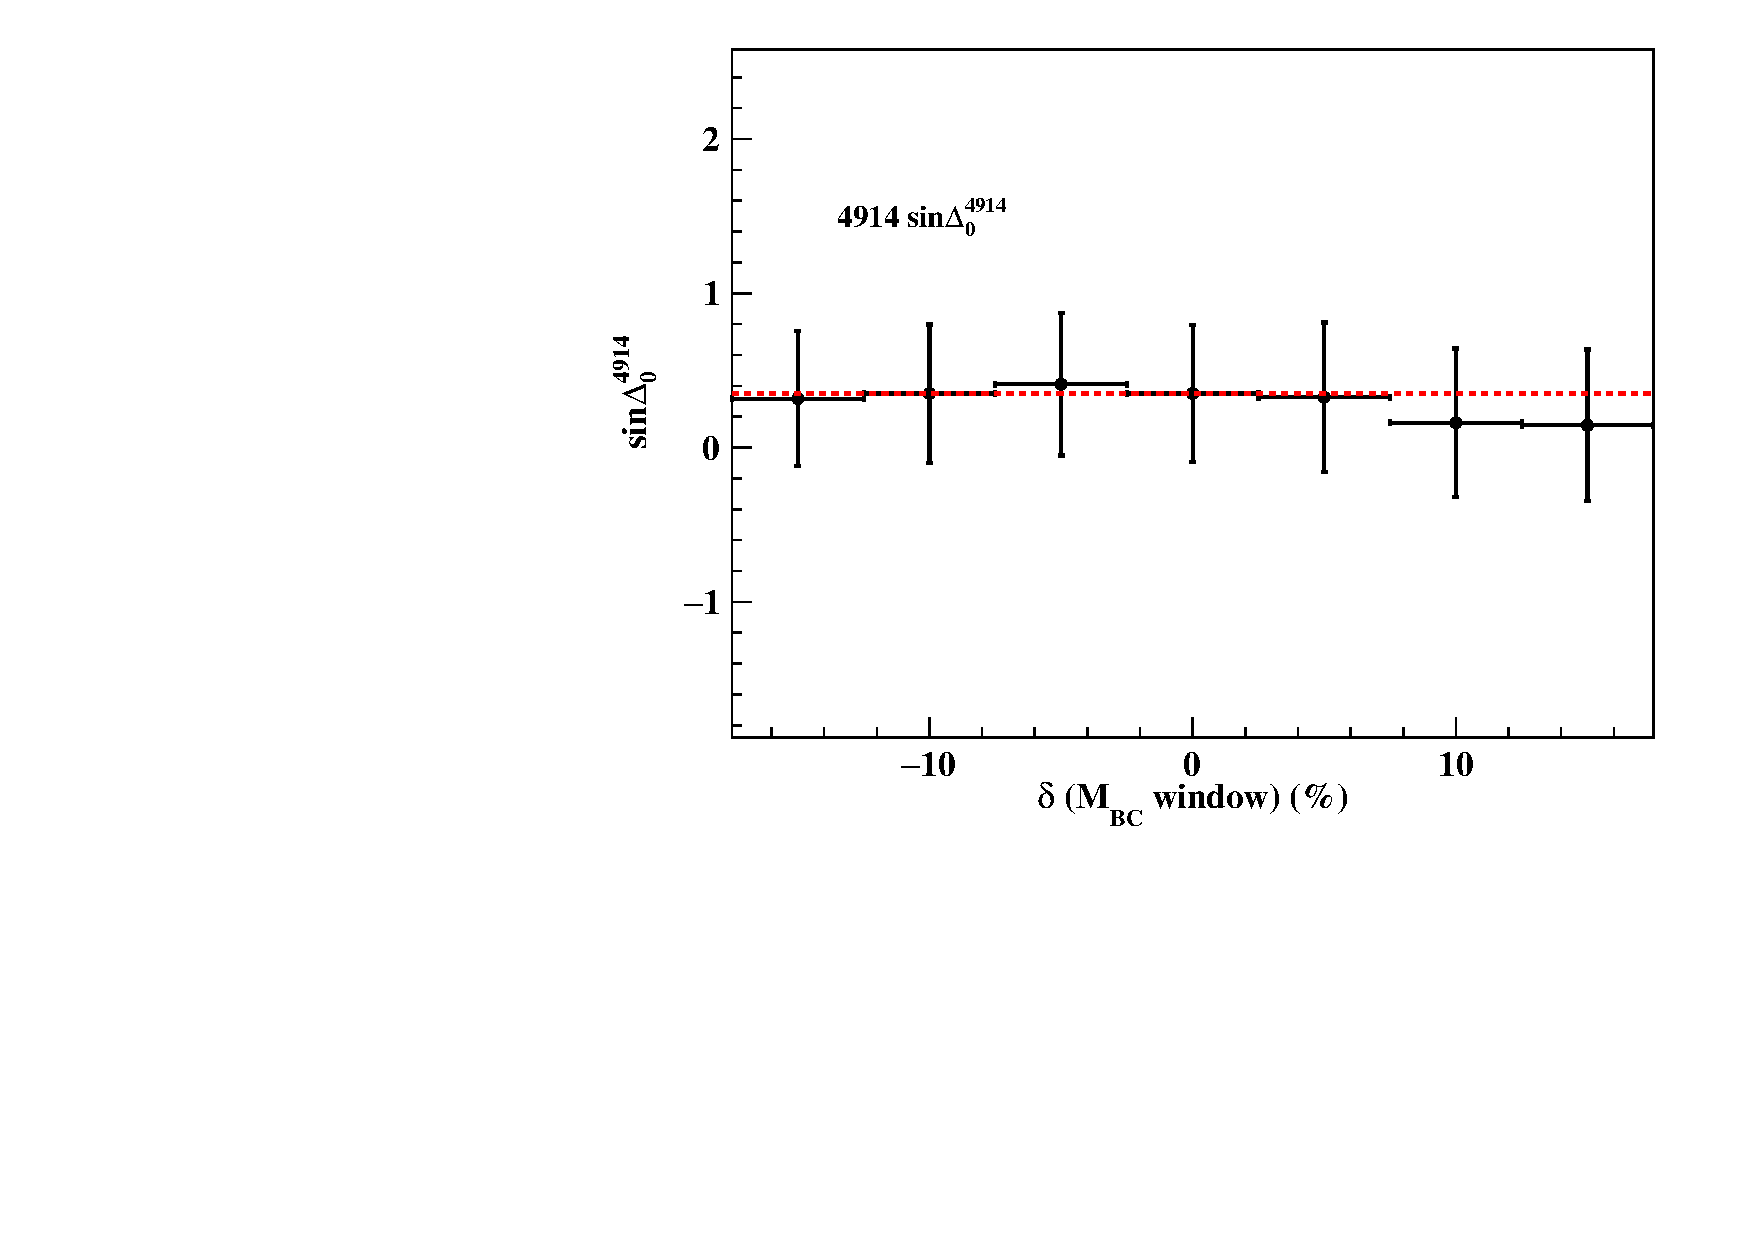
\includegraphics[width=0.40\textwidth]{figure/isr_effects/pwa_fit/output_resutls_mBC_delta_4914.pdf} \\
    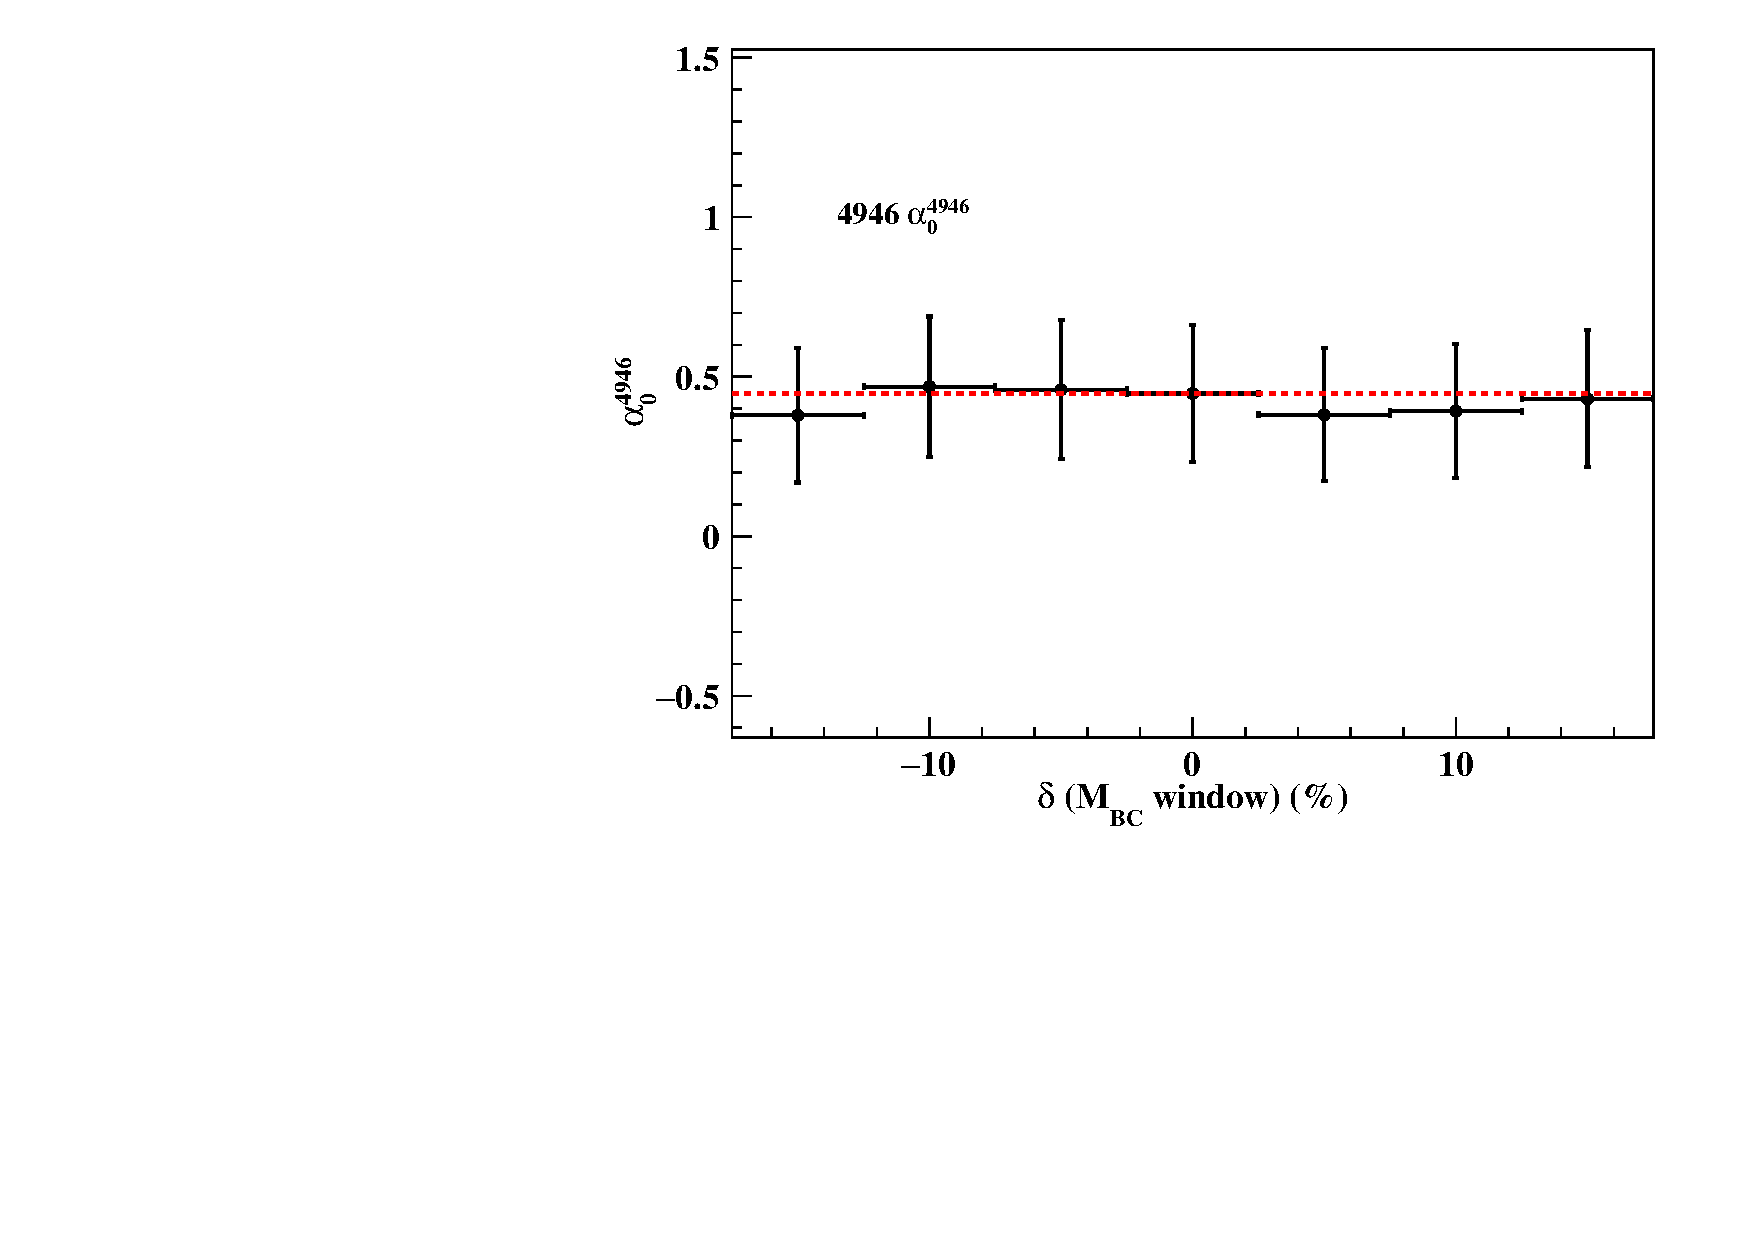
\includegraphics[width=0.40\textwidth]{figure/isr_effects/pwa_fit/output_resutls_mBC_alpha_4946.pdf}
    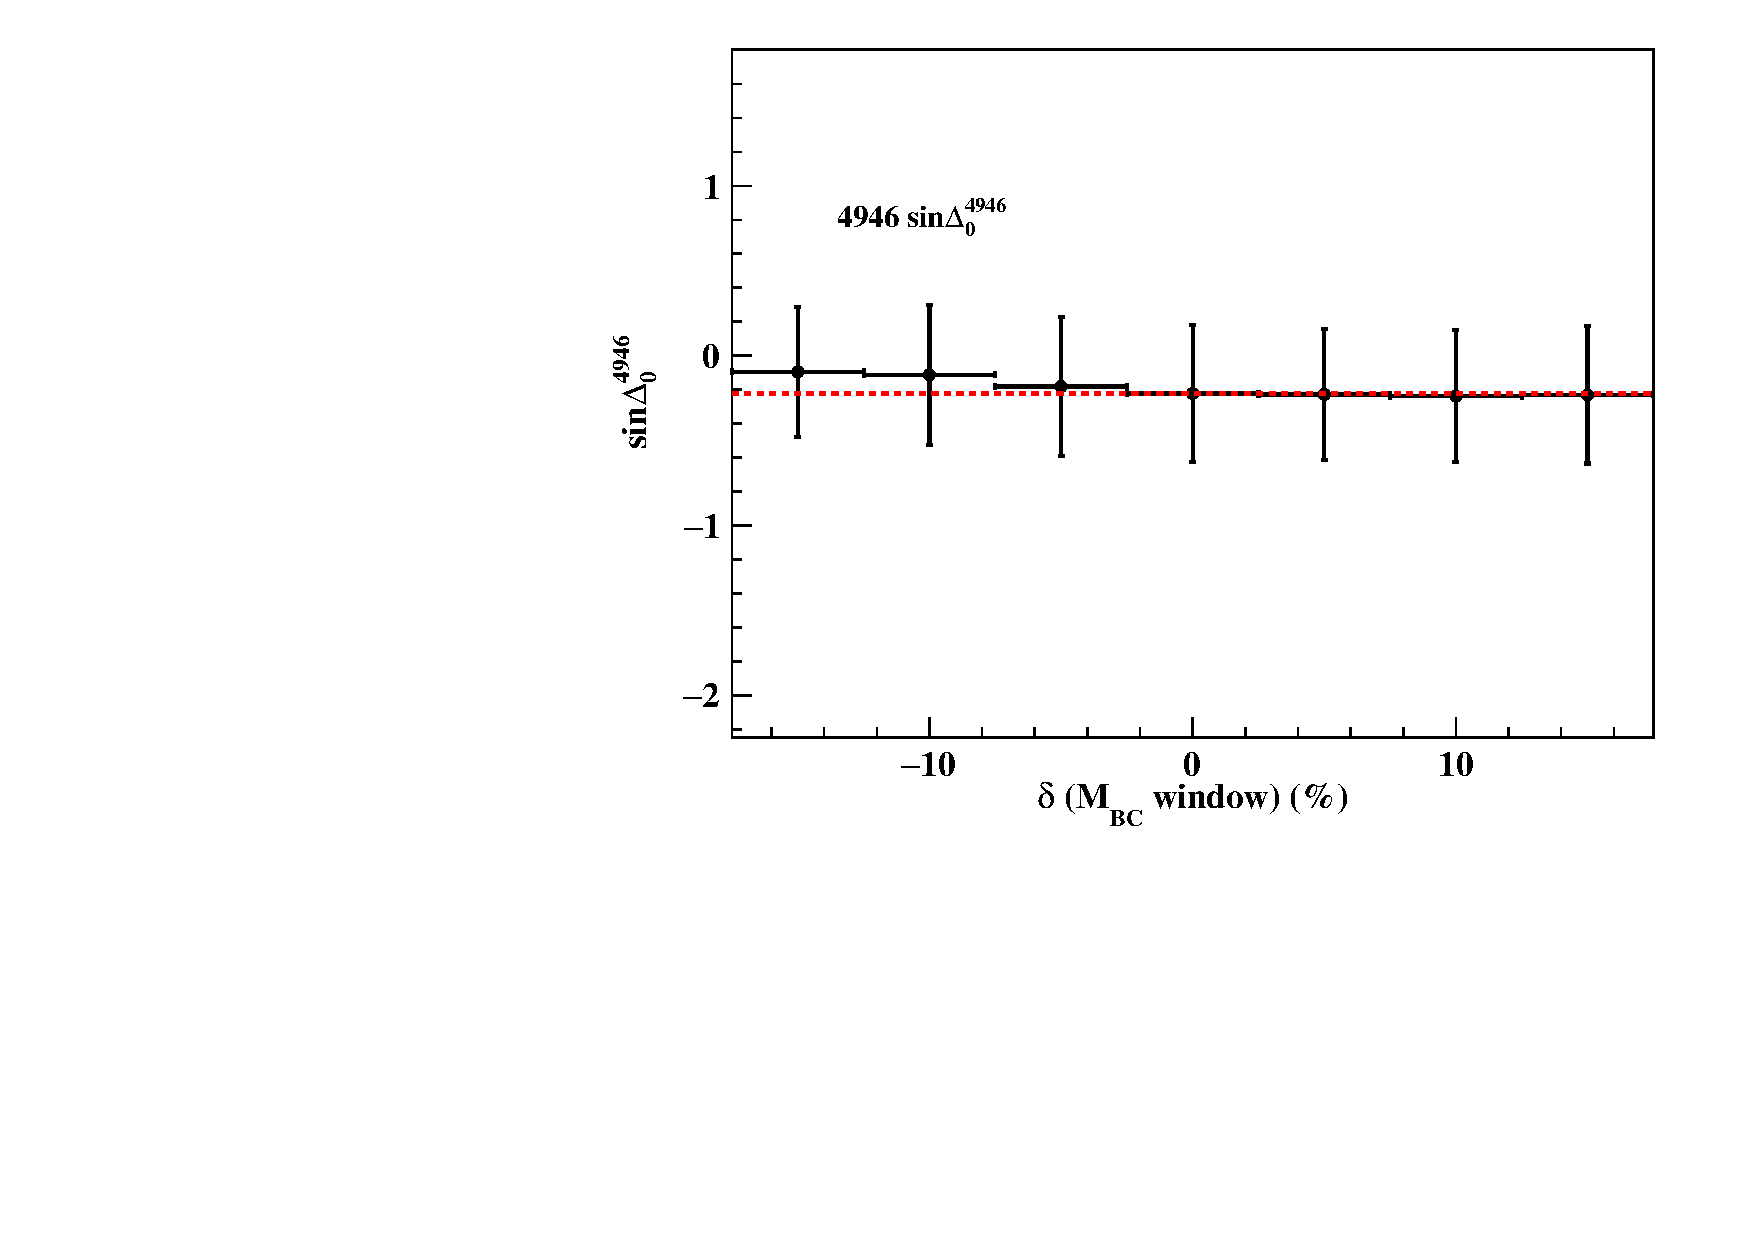
\includegraphics[width=0.40\textwidth]{figure/isr_effects/pwa_fit/output_resutls_mBC_delta_4946.pdf}
    \caption{Comparison of $\alpha_0$ (left) and $\sin\Delta_0$ between nominal and alternative $\mbc$ requirements at $sqrt{s} = 4.918\gev/c^2$ (top) and $\sqrt{s} = 4.950\gev/c^2$ (bottom). The middle points represent the nominal results and error bars are statistical uncertainties.}
\label{fig:comparison_mBC}
\end{figure}